\begin{enumerate}[label=\thesubsection.\arabic*, ref=\thesubsection.\theenumi]

    \item If $A$ is a square matrix of order 2 and $|A| = 4$, then find the value of $|2 \cdot AA'|$, where $A'$ is the transpose of matrix $A$.
\par\hfill (12, 2018)\par
\solution All three properties in \eqref{eq:EE26BTECH11225-det} are used, with $n = 2$ and $k = 2$. First, taking the scalar out of a $2 \times 2$ determinant gives the factor $k^n = 2^2$:
\begin{align*}
|2 \cdot AA'| = 2^2\,|AA'| = 4\,|AA'|
\end{align*}
Next, the determinant of a product is the product of determinants, and $|A'| = |A|$:
\begin{align*}
4\,|AA'| = 4\,|A|\,|A'| = 4\,|A|^2
\end{align*}
Substituting $|A| = 4$,
\begin{align}
|2 \cdot AA'| = 4 \times 4^2 = \boxed{64}
\end{align}
    \item
    \begin{enumerate}[label=(\alph*), leftmargin=1.5em, labelsep=0.5em]
        \item Find the angle between the line $\vec{r} = \myvec{2 \\ -1 \\ 3} + \lambda\myvec{3 \\ -1 \\ 2}$ and the plane $\vec{r}\cdot\myvec{1 \\ 1 \\ 1} = 3$.

        \begin{center}
            \textbf{OR}
        \end{center}

        \item Find the co-ordinates of the point, where the line $\dfrac{x+2}{1} = \dfrac{y-5}{3} = \dfrac{z+1}{5}$ cuts the $yz$-plane.
    \end{enumerate} \vspace{2pt}

\par\hfill (12, 2018)\par
\textbf{(a) Solution:} The line has direction $\vec{b} = \myvec{3 \\ -1 \\ 2}$ and the plane has normal $\vec{n} = \myvec{1 \\ 1 \\ 1}$. The quantities needed in \eqref{eq:EE26BTECH11225-lineplane} are
\begin{align*}
\vec{b}^{\top}\vec{n} &= 3(1) + (-1)(1) + 2(1) = 4 \\
\norm{\vec{b}} = \sqrt{9 + 1 + 4} = \sqrt{14}, &\quad
\norm{\vec{n}} = \sqrt{1 + 1 + 1} = \sqrt{3}
\end{align*}
Substituting,
\begin{align}
\sin\theta = \frac{\left|\vec{b}^{\top}\vec{n}\right|}{\norm{\vec{b}}\norm{\vec{n}}} = \frac{4}{\sqrt{14}\sqrt{3}} = \frac{4}{\sqrt{42}}
\end{align}
so
\begin{align}
\boxed{\theta = \sin^{-1}\frac{4}{\sqrt{42}} \approx 38.1^\circ}
\end{align}
\textbf{(b) Solution:} Setting each ratio equal to $\lambda$ gives $x = -2 + \lambda$, $y = 5 + 3\lambda$, $z = -1 + 5\lambda$, that is
\begin{align*}
\vec{x} = \myvec{-2 \\ 5 \\ -1} + \lambda\myvec{1 \\ 3 \\ 5}
\end{align*}
Every point of the $yz$-plane has $x = 0$, so $-2 + \lambda = 0$, giving $\lambda = 2$. Substituting back,
\begin{align}
\vec{x} = \myvec{-2 \\ 5 \\ -1} + 2\myvec{1 \\ 3 \\ 5} = \myvec{-2 + 2 \\ 5 + 6 \\ -1 + 10} = \boxed{\myvec{0 \\ 11 \\ 9}}
\end{align}
Both parts are plotted in \figref{fig:lineplane_q2}.
\codedesc{2.2.2.py}{Computes $\sin\theta$ from $\vec{b}$ and $\vec{n}$, finds where the line meets $x = 0$, and draws both parts in 3D.}
\begin{lstlisting}[frame=single, basicstyle=\rmfamily, escapeinside={(*@}{@*)}]
(*@\makebox[\dimexpr\linewidth-2\fboxsep-2\fboxrule\relax][c]{codes/2.2.2.py}@*)
\end{lstlisting}
\begin{figure}[H]
    \centering
    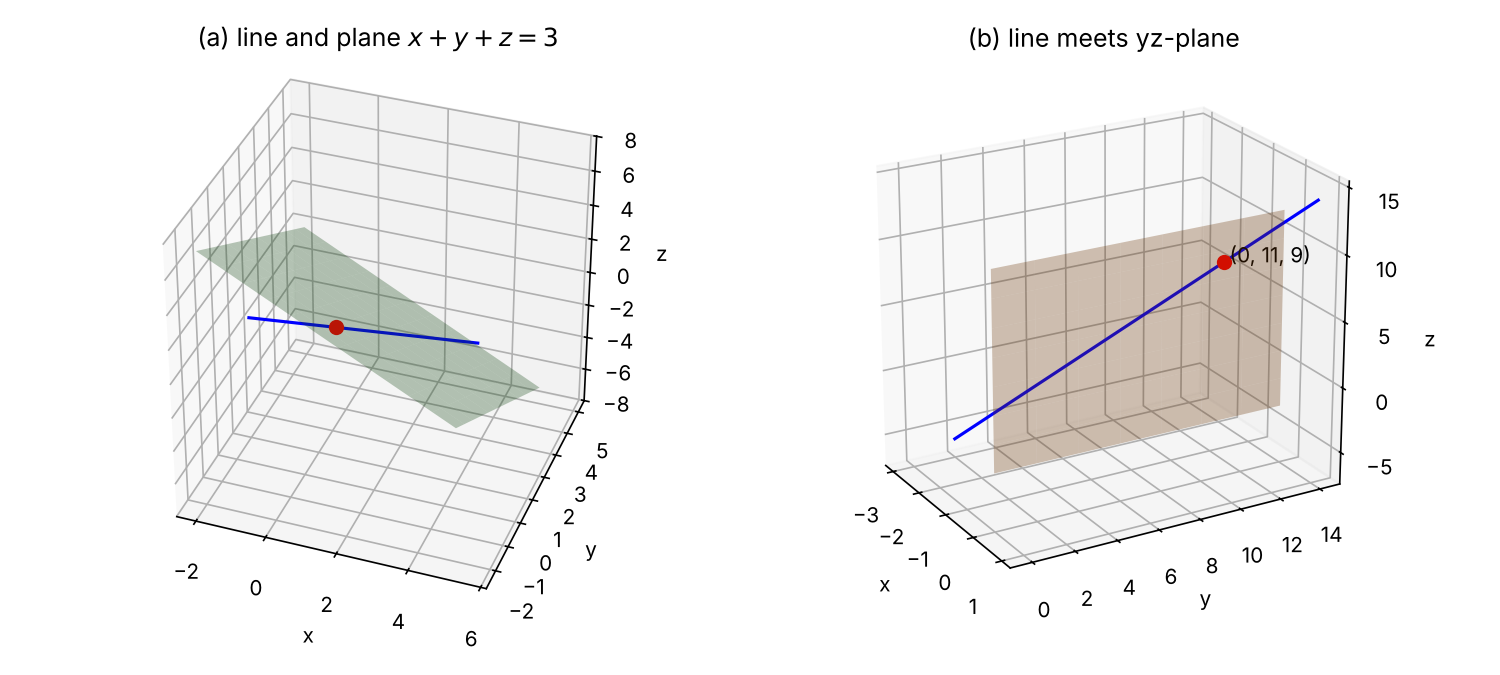
\includegraphics[width=\linewidth]{figs/2.2.2.png}
    \caption{The line and the plane}
    \label{fig:lineplane_q2}
\end{figure}
    \item If an operation $*$ on the set of integers $\mathbb{Z}$ is defined by $a * b = 2a^2 + b$, then find (i) whether it is a binary or not, and (ii) if a binary, then is it commutative or not.
\par\hfill (12, 2018)\par
\solution (i) For any $a, b\in\mathbb{Z}$, $a^2$ is an integer, so $2a^2$ is an integer and $2a^2+b\in\mathbb{Z}$. Thus $*$ maps $\mathbb{Z}\times\mathbb{Z}\to\mathbb{Z}$ and is a binary operation. \\[4pt]
(ii) From \eqref{eq:EE26BTECH11225-binop}, $*$ is commutative only if $a * b = b * a$ for every pair. Here
\begin{align*}
    a * b = 2a^2 + b, \quad b * a = 2b^2 + a
\end{align*}
which are different in general. A single counterexample is enough; take $a=1$, $b=2$:
\begin{align}
    1 * 2 = 2(1)^2 + 2 = 4, \quad 2 * 1 = 2(2)^2 + 1 = 9 \implies 1*2 \neq 2*1
\end{align}
Hence $*$ is a binary operation but it is \textbf{not commutative}.
    \item
    \begin{enumerate}[label=(\alph*), leftmargin=1.5em, labelsep=0.5em]
        \item Four cards are drawn one by one with replacement from a well-shuffled deck of playing cards. Find the probability that at least three cards are of diamonds.

        \begin{center}
            \textbf{OR}
        \end{center}

        \item The probability of two students $A$ and $B$ coming to school on time are $\frac{2}{7}$ and $\frac{4}{7}$, respectively. Assuming that the events `$A$ coming on time' and `$B$ coming on time' are independent, find the probability of only one of them coming to school on time.
    \end{enumerate} \vspace{2pt}

\par\hfill (12, 2018)\par
\textbf{(a) Solution:} Let $X$ be the number of diamonds in $4$ draws. There are $13$ diamonds in $52$ cards, so each draw gives a diamond with probability $\frac{13}{52} = \frac{1}{4}$, and the draws are independent because the card is replaced. So $X$ is binomial with pmf
\begin{align}
p_X(r) = \binom{4}{r}\brak{\frac{1}{4}}^r\brak{\frac{3}{4}}^{4-r}, \quad r = 0, 1, \ldots, 4
\end{align}
The two values needed are
\begin{align*}
p_X(3) = \binom{4}{3}\brak{\frac{1}{4}}^3\brak{\frac{3}{4}} = 4 \cdot \frac{1}{64} \cdot \frac{3}{4} = \frac{12}{256}, \quad
p_X(4) = \brak{\frac{1}{4}}^4 = \frac{1}{256}
\end{align*}
From \eqref{eq:12-pmf}, ``at least three'' is the event $\{3, 4\}$, so
\begin{align}
\Pr\brak{X \geq 3} = p_X(3) + p_X(4) = \frac{12}{256} + \frac{1}{256} = \boxed{\frac{13}{256}}
\end{align}
\textbf{(b) Solution:} Let $a = 1$ if $A$ is on time and $a = 0$ if not, and similarly $b$ for $B$. Then $\Pr(a = 0) = 1 - \frac{2}{7} = \frac{5}{7}$ and $\Pr(b = 0) = 1 - \frac{4}{7} = \frac{3}{7}$. Since the events are independent, from \eqref{eq:12-pmf-sum} the joint pmf is
\begin{align}
p(a, b) = \brak{\frac{2}{7}}^a\brak{\frac{5}{7}}^{1-a}\brak{\frac{4}{7}}^b\brak{\frac{3}{7}}^{1-b}, \quad a, b \in \{0, 1\}
\end{align}
``Only one on time'' is $Z = a + b = 1$, which happens for $(a,b) = (1,0)$ or $(0,1)$:
\begin{align*}
p(1,0) = \frac{2}{7}\cdot\frac{3}{7} = \frac{6}{49}, \quad p(0,1) = \frac{5}{7}\cdot\frac{4}{7} = \frac{20}{49}
\end{align*}
Adding them, from \eqref{eq:12-pmf},
\begin{align}
\Pr\brak{Z = 1} = \frac{6}{49} + \frac{20}{49} = \boxed{\frac{26}{49}}
\end{align}
The stem plots in \figref{fig:pmf_q4} compare the simulated and theoretical pmfs.
\codedesc{2.2.4.py}{Simulates $10^6$ trials of each part and compares the simulated pmfs with the binomial pmf of $X$ and the pmf of $Z$.}
\begin{lstlisting}[frame=single, basicstyle=\rmfamily, escapeinside={(*@}{@*)}]
(*@\makebox[\dimexpr\linewidth-2\fboxsep-2\fboxrule\relax][c]{codes/2.2.4.py}@*)
\end{lstlisting}
\begin{figure}[H]
    \centering
    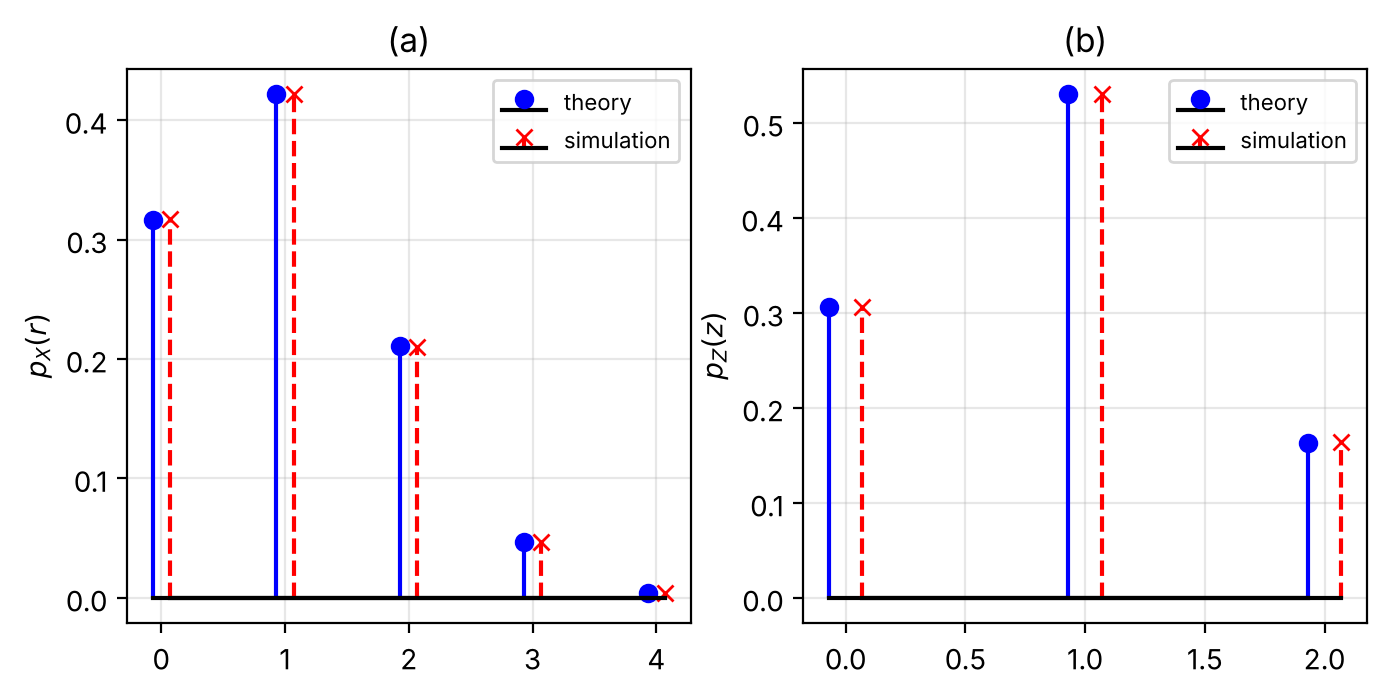
\includegraphics[width=\linewidth]{figs/2.2.4.png}
    \caption{Theoretical and simulated pmfs: (a) $p_X(r)$, (b) $p_Z(z)$}
    \label{fig:pmf_q4}
\end{figure}
    \item
    \begin{enumerate}[label=(\alph*), leftmargin=1.5em, labelsep=0.5em]
        \item Using vectors, prove that the points $(2,-1,3)$, $(3,-5,1)$ and $(-1,11,9)$ are collinear.

        \begin{center}
            \textbf{OR}
        \end{center}

        \item For any two vectors $\vec{a}$ and $\vec{b}$, prove that $(\vec{a}\times\vec{b})^2 = \vec{a}^2\vec{b}^2 - (\vec{a}\cdot\vec{b})^2$.
    \end{enumerate} \vspace{2pt}

\par\hfill (12, 2018)\par
\textbf{(a) Solution:} Let $A(2,-1,3)$, $B(3,-5,1)$, $C(-1,11,9)$. Then
\begin{align*}
    \vec{AB} &= \myvec{3-2 \\ -5+1 \\ 1-3} = \myvec{1 \\ -4 \\ -2} \\
    \vec{BC} &= \myvec{-1-3 \\ 11+5 \\ 9-1} = \myvec{-4 \\ 16 \\ 8} = -4\myvec{1 \\ -4 \\ -2}
\end{align*}
so
\begin{align}
\vec{BC} = -4\,\vec{AB}
\end{align}
The two vectors are parallel, and they share the point $B$, so they lie on the same line. Hence $A$, $B$, $C$ are collinear. \\[8pt]
\textbf{(b) Solution:} Let $\theta$ be the angle between $\vec{a}$ and $\vec{b}$. Squaring \eqref{eq:EE26BTECH11225-cross} and using $\sin^2\theta = 1 - \cos^2\theta$,
\begin{align*}
    \|\vec{a}\times\vec{b}\|^2 &= \|\vec{a}\|^2\|\vec{b}\|^2\sin^2\theta \\
    &= \|\vec{a}\|^2\|\vec{b}\|^2\left(1-\cos^2\theta\right) \\
    &= \|\vec{a}\|^2\|\vec{b}\|^2 - \left(\|\vec{a}\|\|\vec{b}\|\cos\theta\right)^2
\end{align*}
From \eqref{eq:EE26BTECH11225-dot}, $\|\vec{a}\|\|\vec{b}\|\cos\theta = \vec{a}^{\top}\vec{b}$. Substituting this in the last term,
\begin{align}
    \|\vec{a}\times\vec{b}\|^2 = \|\vec{a}\|^2\|\vec{b}\|^2 - \left(\vec{a}^{\top}\vec{b}\right)^2
\end{align}
which is the required identity. The points are plotted in \figref{fig:collinear_q6}.
\codedesc{2.2.6.py}{Checks $\vec{BC} = -4\,\vec{AB}$ and that $\sbrak{\vec{AB}\ \vec{BC}}$ has rank $1$, verifies the identity numerically, and plots the points in 3D.}
\begin{lstlisting}[frame=single, basicstyle=\rmfamily, escapeinside={(*@}{@*)}]
(*@\makebox[\dimexpr\linewidth-2\fboxsep-2\fboxrule\relax][c]{codes/2.2.6.py}@*)
\end{lstlisting}
\begin{figure}[H]
    \centering
    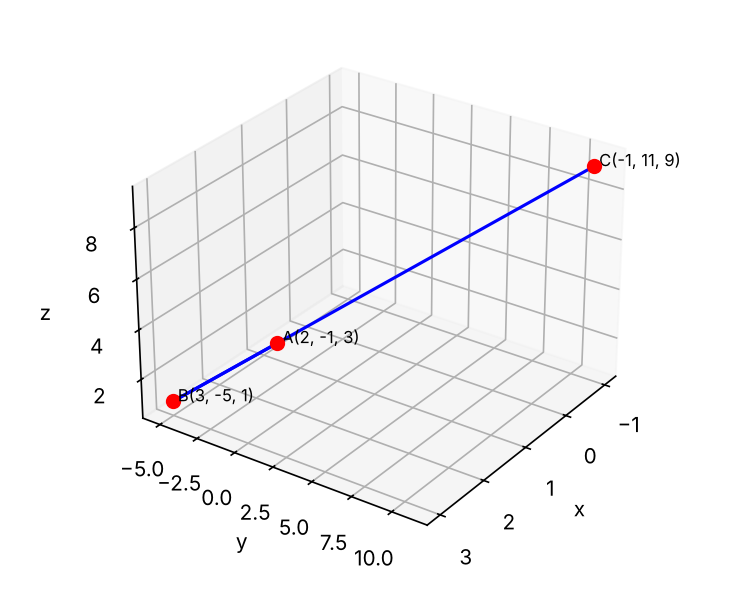
\includegraphics[width=0.75\linewidth]{figs/2.2.6.png}
    \caption{The collinear points $A$, $B$, $C$}
    \label{fig:collinear_q6}
\end{figure}
    \item If $A$ and $B$ are independent events with $P(A) = \frac{3}{7}$ and $P(B) = \frac{2}{5}$, then find $P(A'\cap B')$.
\par\hfill (12, 2018)\par
\solution
Let $I_A$ and $I_B$ be the indicators of $A$ and $B$ ($1$ if the event happens, $0$ if not). Then
\begin{align*}
\Pr\brak{I_A = 0} = 1 - \frac{3}{7} = \frac{4}{7}, \quad \Pr\brak{I_B = 0} = 1 - \frac{2}{5} = \frac{3}{5}
\end{align*}
Being independent, their joint pmf from \eqref{eq:12-pmf-sum} is the product
\begin{align}
p(a,b) = \brak{\frac{3}{7}}^a\brak{\frac{4}{7}}^{1-a}\brak{\frac{2}{5}}^b\brak{\frac{3}{5}}^{1-b}, \quad a, b \in \{0, 1\}
\end{align}
The event $A' \cap B'$ means neither event happens, that is $a = b = 0$:
\begin{align}
\Pr\brak{A' \cap B'} = p(0,0) = \frac{4}{7}\cdot\frac{3}{5} = \boxed{\frac{12}{35}}
\end{align}
The simulated pmf is compared with $p(a,b)$ in \figref{fig:pmf_q7}.
\codedesc{2.2.7.py}{Simulates $10^6$ pairs of independent indicators and compares the simulated joint pmf with $p(a, b)$.}
\begin{lstlisting}[frame=single, basicstyle=\rmfamily, escapeinside={(*@}{@*)}]
(*@\makebox[\dimexpr\linewidth-2\fboxsep-2\fboxrule\relax][c]{codes/2.2.7.py}@*)
\end{lstlisting}
\begin{figure}[H]
    \centering
    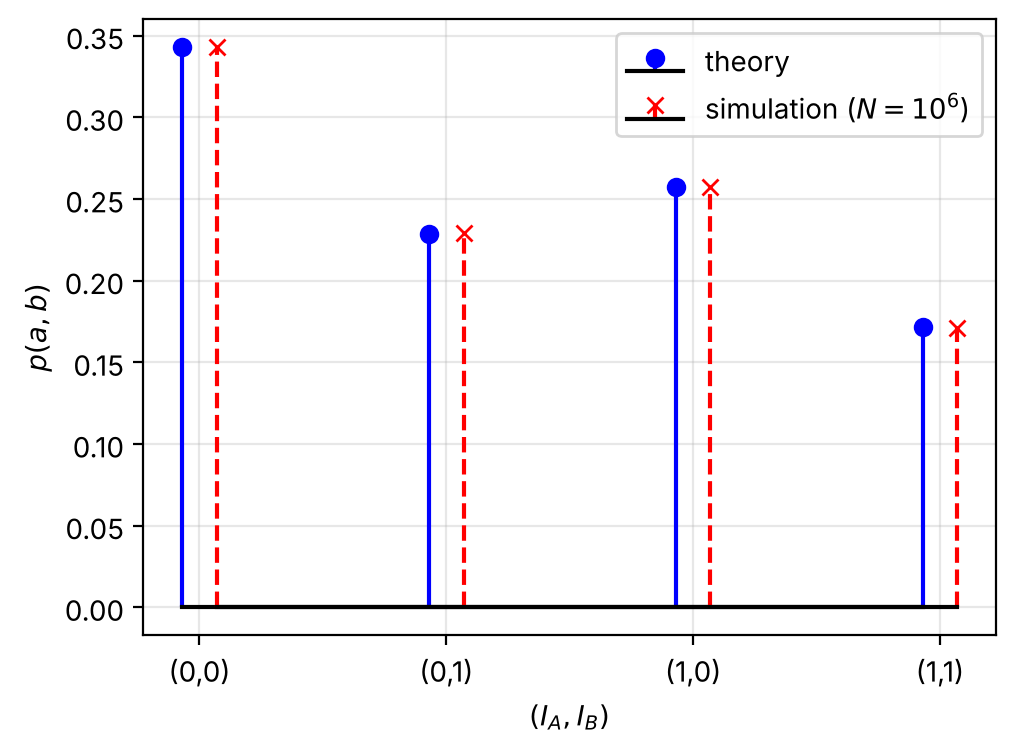
\includegraphics[width=0.8\linewidth]{figs/2.2.7.png}
    \caption{Theoretical and simulated $p(a,b)$}
    \label{fig:pmf_q7}
\end{figure}
    \item Find the equation of the plane passing through the point $(-1,3,2)$ and perpendicular to the planes $x+2y+3z=5$ and $3x+3y+z=0$.
\par\hfill (12, 2018)\par
\solution
Since the required plane is perpendicular to both given planes, its normal $\vec{n}$ is perpendicular to both of their normals $\vec{n}_1 = \myvec{1 \\ 2 \\ 3}$ and $\vec{n}_2 = \myvec{3 \\ 3 \\ 1}$, that is
\begin{align}
\myvec{1 & 2 & 3 \\ 3 & 3 & 1}\vec{n} = \vec{0}
\end{align}
Gauss elimination \eqref{eq:EE26BTECH11225-gauss-mult} with the multiplier $m_{21} = 3$ gives
\begin{align*}
\myvec{1 & 2 & 3 \\ 3 & 3 & 1} \xrightarrow{R_2 \to R_2 - 3R_1} \myvec{1 & 2 & 3 \\ 0 & -3 & -8}
\end{align*}
There are two equations in three unknowns, so $n_3$ is free. Taking $n_3 = 3$ and back-substituting,
\begin{align*}
-3n_2 - 8(3) = 0 &\implies n_2 = -8 \\
n_1 + 2(-8) + 3(3) = 0 &\implies n_1 = 7
\end{align*}
so $\vec{n} = \myvec{7 \\ -8 \\ 3}$. The plane through $\vec{p} = \myvec{-1 \\ 3 \\ 2}$ is, from \eqref{eq:EE26BTECH11225-plane},
\begin{align*}
7(x + 1) - 8(y - 3) + 3(z - 2) = 0
\end{align*}
Expanding, $7x - 8y + 3z + 7 + 24 - 6 = 0$, that is
\begin{align}
\boxed{7x - 8y + 3z + 25 = 0}
\end{align}
The three planes are plotted in \figref{fig:plane_q8}.
\codedesc{2.2.8.py}{Does the elimination on $\sbrak{\vec{n}_1\ \vec{n}_2}^{\top}$, back-substitutes with $n_3 = 3$, prints the plane and plots the three planes.}
\begin{lstlisting}[frame=single, basicstyle=\rmfamily, escapeinside={(*@}{@*)}]
(*@\makebox[\dimexpr\linewidth-2\fboxsep-2\fboxrule\relax][c]{codes/2.2.8.py}@*)
\end{lstlisting}
\begin{figure}[H]
    \centering
    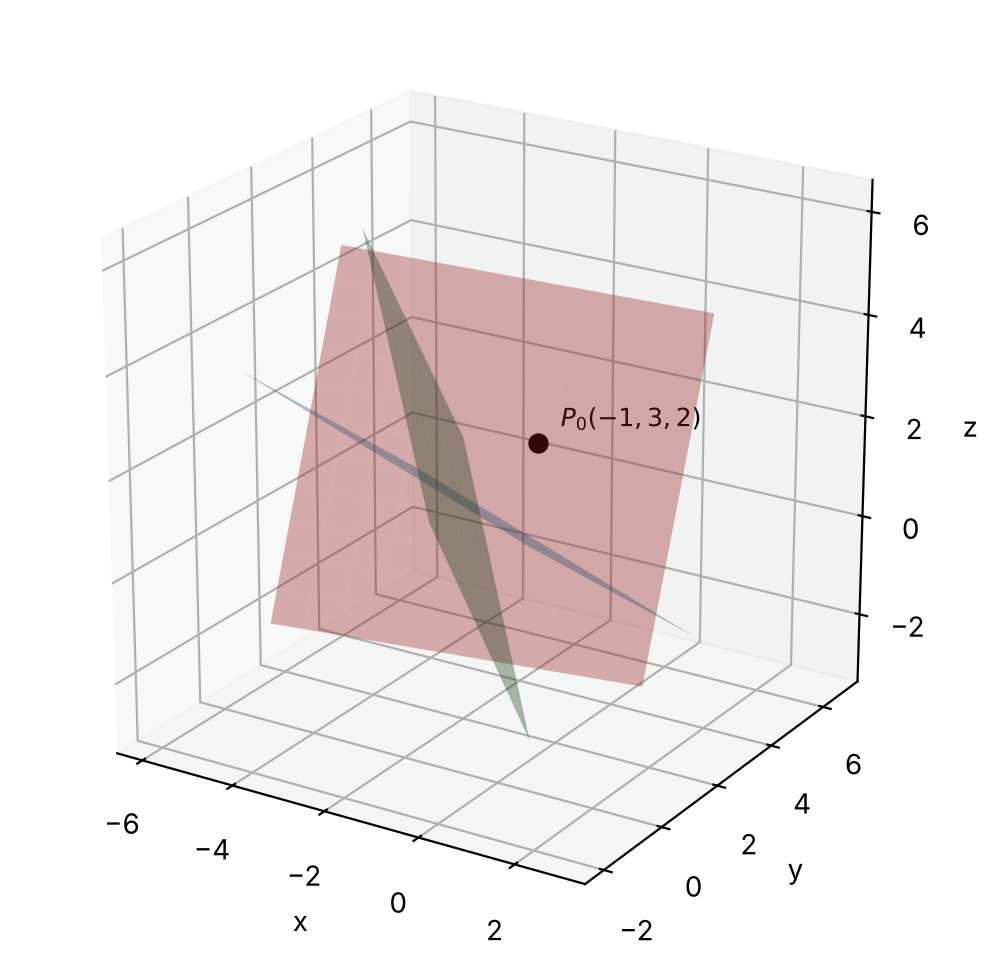
\includegraphics[width=0.7\linewidth]{figs/2.2.8.png}
    \caption{The given planes and the required plane}
    \label{fig:plane_q8}
\end{figure}
    \item Evaluate: $\displaystyle\int_1^5 \big(|x-1| + |x-2| + |x-4|\big)\,dx$
\par\hfill (12, 2018)\par
\solution
Let $g(x) = |x-1| + |x-2| + |x-4|$. Each term changes slope only where its inside is zero, so $g$ has corners only at $x = 1, 2, 4$ and is a straight line in between. Take $h = 1$ ($N = 4$, nodes $1, 2, 3, 4, 5$). Every corner is a node, so $g$ is linear between nodes and the trapezoidal rule is exact. The values at the nodes are
\begin{align*}
g(1) &= 0 + 1 + 3 = 4, & g(2) &= 1 + 0 + 2 = 3, & g(3) &= 2 + 1 + 1 = 4, \\
g(4) &= 3 + 2 + 0 = 5, & g(5) &= 4 + 3 + 1 = 8
\end{align*}
From \eqref{eq:EE26BTECH11225-trapezoid} with $h = 1$,
\begin{align}
\int_1^5 g(x)\,dx &= \frac{1}{2}\sbrak{g(1) + 2g(2) + 2g(3) + 2g(4) + g(5)} \nonumber \\
&= \frac{1}{2}\sbrak{4 + 2(3+4+5) + 8} = \frac{36}{2} = \boxed{18}
\end{align}
Both $N = 4$ and $N = 1000$ give $18$. The trapezoids are drawn in \figref{fig:trap_q9}.
\codedesc{2.2.9.c}{Applies the trapezoidal rule with $N = 4$ and $N = 1000$ and prints both results.}
\begin{lstlisting}[frame=single, basicstyle=\rmfamily, escapeinside={(*@}{@*)}]
(*@\makebox[\dimexpr\linewidth-2\fboxsep-2\fboxrule\relax][c]{codes/2.2.9.c}@*)
\end{lstlisting}
\codedesc{2.2.9.py}{Repeats the rule with $N = 4$ and shades the four trapezoids under $g(x)$.}
\begin{lstlisting}[frame=single, basicstyle=\rmfamily, escapeinside={(*@}{@*)}]
(*@\makebox[\dimexpr\linewidth-2\fboxsep-2\fboxrule\relax][c]{codes/2.2.9.py}@*)
\end{lstlisting}
\begin{figure}[H]
    \centering
    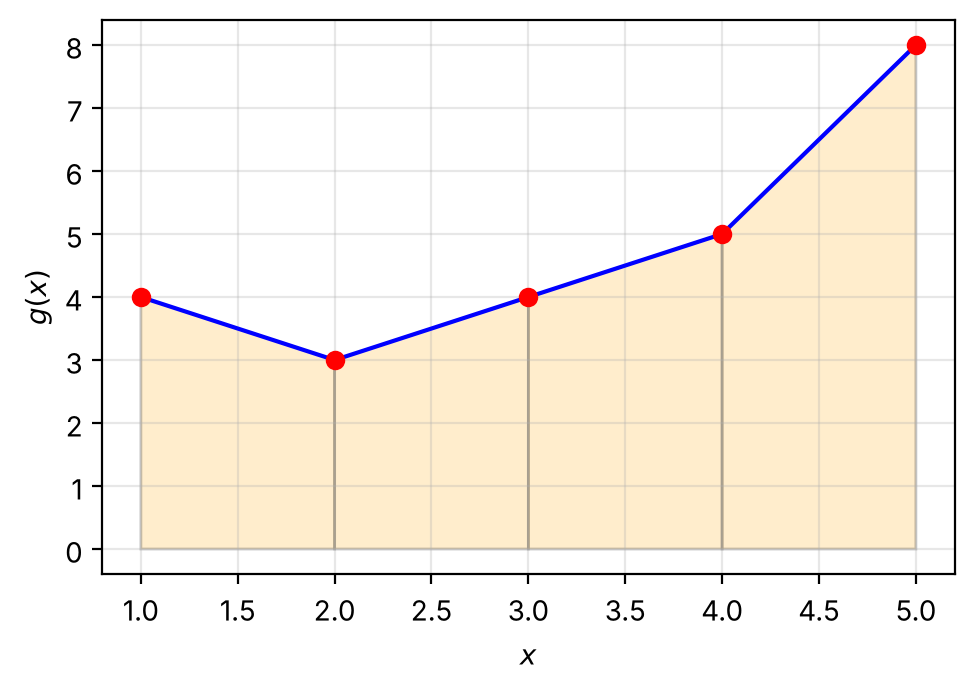
\includegraphics[width=0.8\linewidth]{figs/2.2.9.png}
    \caption{The trapezoids for $N = 4$}
    \label{fig:trap_q9}
\end{figure}
    \item If $x,y,z$ are different and $\Delta = \begin{vmatrix} x & x^2 & x^3-1 \\ y & y^2 & y^3-1 \\ z & z^2 & z^3-1 \end{vmatrix} = 0$, then using properties of determinants, show that $xyz=1$.
\par\hfill (12, 2018)\par

\solution
From \eqref{eq:EE26BTECH11225-vieta}, $\Delta = 0$ means the columns of the matrix are linearly dependent: there is $\vec{c} = \myvec{\alpha \\ \beta \\ \gamma} \neq \vec{0}$ with
\begin{align}
\myvec{x & x^2 & x^3 - 1 \\ y & y^2 & y^3 - 1 \\ z & z^2 & z^3 - 1}\myvec{\alpha \\ \beta \\ \gamma} = \vec{0}
\end{align}
Reading off any row, say the first, $\alpha x + \beta x^2 + \gamma\brak{x^3 - 1} = 0$. The other rows are the same with $y$ and $z$. So each of $t = x, y, z$ satisfies
\begin{align*}
\gamma t^3 + \beta t^2 + \alpha t - \gamma = 0
\end{align*}
If $\gamma = 0$, this is at most quadratic, so it cannot have three distinct roots unless $\alpha = \beta = 0$, which contradicts $\vec{c} \neq \vec{0}$. Hence $\gamma \neq 0$, and $x, y, z$ are the three roots of a cubic whose constant term is $\delta = -\gamma$. From \eqref{eq:EE26BTECH11225-vieta}, the product of the roots is
\begin{align}
xyz = -\frac{\delta}{\gamma} = -\frac{-\gamma}{\gamma} = \boxed{1}
\end{align}
An example cubic with its three roots is plotted in \figref{fig:vieta_q10}.
\codedesc{2.2.10.py}{Takes $x = 2$, $y = 3$, builds the cubic with $xyz = 1$, finds $\vec{c}$ with $\vec{M}\vec{c} = \vec{0}$, checks that the rank is $2$ and plots the cubic.}
\begin{lstlisting}[frame=single, basicstyle=\rmfamily, escapeinside={(*@}{@*)}]
(*@\makebox[\dimexpr\linewidth-2\fboxsep-2\fboxrule\relax][c]{codes/2.2.10.py}@*)
\end{lstlisting}
\begin{figure}[H]
    \centering
    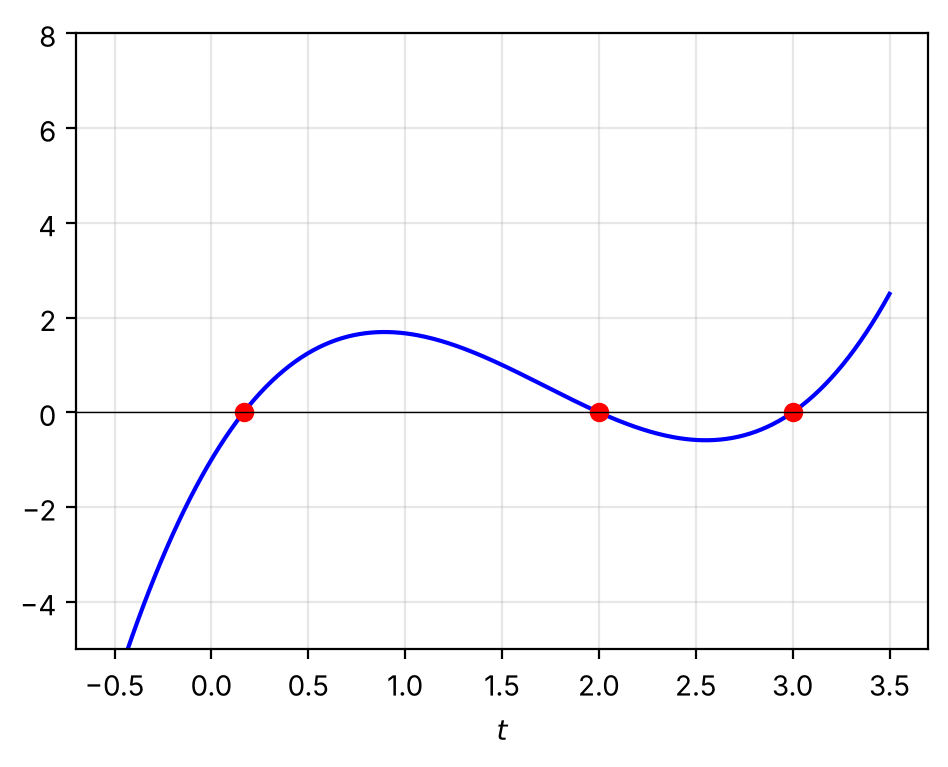
\includegraphics[width=0.75\linewidth]{figs/2.2.10.png}
    \caption{The cubic $t^3 + \beta t^2 + \alpha t - 1$ with roots $x, y, z$ and $xyz = 1$}
    \label{fig:vieta_q10}
\end{figure}
    \item Find the interval in which the function $f$ given by $f(x) = \sin 2x + \cos 2x$, $0\leq x\leq\pi$ is strictly decreasing.
\par\hfill (12, 2018)\par
\solution
Differentiating,
\begin{align}
f'(x) = 2\cos 2x - 2\sin 2x
\end{align}
From \eqref{eq:EE26BTECH11225-mono}, $f$ is strictly decreasing where $f'(x) < 0$. The sign of $f'$ can change only at its zeros, which are found by the Newton--Raphson iteration \eqref{eq:12-newton} applied to $f'$, with $f''(x) = -4\sin 2x - 4\cos 2x$:
\[
\begin{array}{c|r|r}
n & x_n\;(x_0=0.5) & x_n\;(x_0=2)\\\hline
0 & 0.500000 & 2.000000 \\
1 & 0.391021 & 1.963430 \\
2 & 0.392699 & 1.963495 \\
3 & 0.392699 & 1.963495
\end{array}
\]
The limits are $0.392699 = \frac{\pi}{8}$ and $1.963495 = \frac{5\pi}{8}$ (indeed $\tan 2x = 1$ there). Testing one point in each sub-interval,
\begin{align*}
f'(0) = 2 > 0, \quad f'(1) = -2.65 < 0, \quad f'(3) = 2.48 > 0
\end{align*}
so $f'$ is negative only between the two zeros. Hence
\begin{align}
\boxed{f \text{ is strictly decreasing on } \brak{\tfrac{\pi}{8}, \tfrac{5\pi}{8}}}
\end{align}
$f$ and $f'$ are plotted in \figref{fig:decr_q13}.
\codedesc{2.2.13.c}{Runs Newton--Raphson on $f'(x)$ from $x_0 = 0.5$ and $2$ and prints the zeros next to $\frac{\pi}{8}$ and $\frac{5\pi}{8}$.}
\begin{lstlisting}[frame=single, basicstyle=\rmfamily, escapeinside={(*@}{@*)}]
(*@\makebox[\dimexpr\linewidth-2\fboxsep-2\fboxrule\relax][c]{codes/2.2.13.c}@*)
\end{lstlisting}
\codedesc{2.2.13.py}{Evaluates $f'$ on a fine grid to find where it is negative, and plots $f$ and $f'$.}
\begin{lstlisting}[frame=single, basicstyle=\rmfamily, escapeinside={(*@}{@*)}]
(*@\makebox[\dimexpr\linewidth-2\fboxsep-2\fboxrule\relax][c]{codes/2.2.13.py}@*)
\end{lstlisting}
\begin{figure}[H]
    \centering
    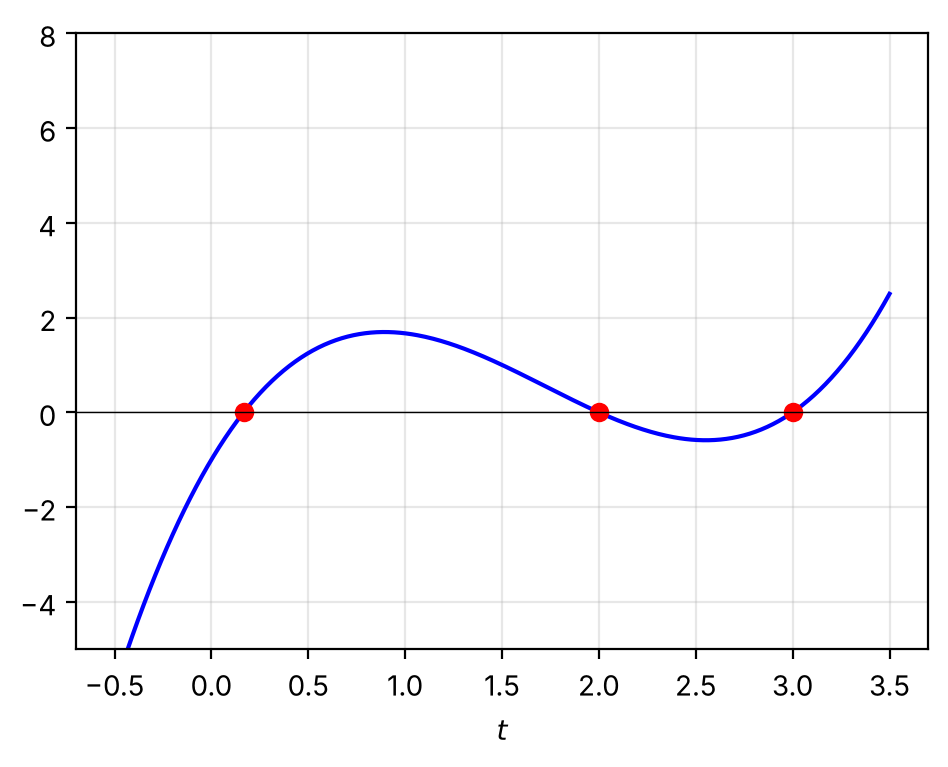
\includegraphics[width=0.9\linewidth]{figs/2.2.13.png}
    \caption{$f(x) = \sin 2x + \cos 2x$ and $f'(x)$}
    \label{fig:decr_q13}
\end{figure}
    \item
    \begin{enumerate}[label=(\alph*), leftmargin=1.5em, labelsep=0.5em]
        \item Using elementary row transformations, find the inverse of the matrix
        \begin{align*}
            \begin{bmatrix} 3 & 0 & -1 \\ 2 & 3 & 0 \\ 0 & 4 & 1 \end{bmatrix}
        \end{align*}

        \begin{center}
            \textbf{OR}
        \end{center}

        \item Using matrices, solve the following system of linear equations:
        \begin{align*}
            2x+3y+10z &= 4 \\
            4x-6y+5z &= 1 \\
            6x+9y-20z &= 2
        \end{align*}
    \end{enumerate} \vspace{2pt}

\par\hfill (12, 2018)\par
\textbf{(a) Solution:} From \eqref{eq:EE26BTECH11225-rowops}, apply row operations to $[A\,|\,I]$ until the left block becomes $I$:
\begin{align*}
    [A|I] &= \left[\begin{array}{ccc|ccc} 3 & 0 & -1 & 1 & 0 & 0 \\ 2 & 3 & 0 & 0 & 1 & 0 \\ 0 & 4 & 1 & 0 & 0 & 1 \end{array}\right] \\
    \xrightarrow{R_1\to R_1-R_2}\; &\left[\begin{array}{ccc|ccc} 1 & -3 & -1 & 1 & -1 & 0 \\ 2 & 3 & 0 & 0 & 1 & 0 \\ 0 & 4 & 1 & 0 & 0 & 1 \end{array}\right] \\
    \xrightarrow{R_2\to R_2-2R_1}\; &\left[\begin{array}{ccc|ccc} 1 & -3 & -1 & 1 & -1 & 0 \\ 0 & 9 & 2 & -2 & 3 & 0 \\ 0 & 4 & 1 & 0 & 0 & 1 \end{array}\right] \\
    \xrightarrow{R_2\to R_2-2R_3}\; &\left[\begin{array}{ccc|ccc} 1 & -3 & -1 & 1 & -1 & 0 \\ 0 & 1 & 0 & -2 & 3 & -2 \\ 0 & 4 & 1 & 0 & 0 & 1 \end{array}\right] \\
    \xrightarrow{R_1\to R_1+3R_2}\; &\left[\begin{array}{ccc|ccc} 1 & 0 & -1 & -5 & 8 & -6 \\ 0 & 1 & 0 & -2 & 3 & -2 \\ 0 & 4 & 1 & 0 & 0 & 1 \end{array}\right] \\
    \xrightarrow{R_3\to R_3-4R_2}\; &\left[\begin{array}{ccc|ccc} 1 & 0 & -1 & -5 & 8 & -6 \\ 0 & 1 & 0 & -2 & 3 & -2 \\ 0 & 0 & 1 & 8 & -12 & 9 \end{array}\right] \\
    \xrightarrow{R_1\to R_1+R_3}\; &\left[\begin{array}{ccc|ccc} 1 & 0 & 0 & 3 & -4 & 3 \\ 0 & 1 & 0 & -2 & 3 & -2 \\ 0 & 0 & 1 & 8 & -12 & 9 \end{array}\right]
\end{align*}
The right block is now the inverse:
\begin{align}
    \boxed{A^{-1} = \begin{bmatrix} 3 & -4 & 3 \\ -2 & 3 & -2 \\ 8 & -12 & 9 \end{bmatrix}}
\end{align}
Check: the first row of $A$ times the first column of $A^{-1}$ is $3(3) + 0(-2) + (-1)(8) = 1$, and similarly $AA^{-1} = I$. \\[8pt]
\textbf{(b) Solution:} Write the system as $A\vec{x}=\vec{b}$ and use Gaussian elimination on $[A\,|\,\vec{b}]$, with the multipliers $m_{21} = \frac{4}{2} = 2$ and $m_{31} = \frac{6}{2} = 3$ of \eqref{eq:EE26BTECH11225-gauss-mult}:
\begin{align*}
    \big[A\,|\,\vec{b}\big] &= \left[\begin{array}{ccc|c} 2 & 3 & 10 & 4 \\ 4 & -6 & 5 & 1 \\ 6 & 9 & -20 & 2 \end{array}\right] \\
    \xrightarrow[R_3\to R_3-3R_1]{R_2\to R_2-2R_1}\; &\left[\begin{array}{ccc|c} 2 & 3 & 10 & 4 \\ 0 & -12 & -15 & -7 \\ 0 & 0 & -50 & -10 \end{array}\right]
\end{align*}
The matrix is already upper triangular. The pivots $2$, $-12$ and $-50$ are all nonzero, so the solution is unique. By back-substitution, from \eqref{eq:EE26BTECH11225-gauss-back},
\begin{align*}
    -50z = -10 &\implies z = \frac{1}{5} \\
    -12y - 15\left(\frac{1}{5}\right) = -7 \implies -12y = -4 &\implies y = \frac{1}{3} \\
    2x + 3\left(\frac{1}{3}\right) + 10\left(\frac{1}{5}\right) = 4 \implies 2x = 1 &\implies x = \frac{1}{2}
\end{align*}
Hence
\begin{align}
\boxed{x = \frac{1}{2}, \quad y = \frac{1}{3}, \quad z = \frac{1}{5}}
\end{align}
The elimination is coded in C:
\codedesc{2.2.14b.c}{Row-reduces $[A\,|\,\vec{b}]$, prints each stage, back-substitutes and prints the residual $A\vec{x} - \vec{b}$.}
\begin{lstlisting}[frame=single, basicstyle=\rmfamily, escapeinside={(*@}{@*)}]
(*@\makebox[\dimexpr\linewidth-2\fboxsep-2\fboxrule\relax][c]{codes/2.2.14b.c}@*)
\end{lstlisting}
To see how the cost grows with the size $n$ of the system, Gaussian elimination is timed on random $n \times n$ systems. \figref{fig:gauss_time_q14} shows that the time grows as $n^3$, as in \eqref{eq:EE26BTECH11225-gauss-cost}.
\codedesc{2.2.14b\_time.c}{Times Gaussian elimination on random $n \times n$ systems for increasing $n$ and writes the pairs ($n$, seconds) to \texttt{2.2.14b\_time.dat}.}
\begin{lstlisting}[frame=single, basicstyle=\rmfamily, escapeinside={(*@}{@*)}]
(*@\makebox[\dimexpr\linewidth-2\fboxsep-2\fboxrule\relax][c]{codes/2.2.14b\_time.c}@*)
\end{lstlisting}
\codedesc{2.2.14b\_time.py}{Reads \texttt{2.2.14b\_time.dat} and plots the time against $n$ on log-log axes with an $n^3$ reference line.}
\begin{lstlisting}[frame=single, basicstyle=\rmfamily, escapeinside={(*@}{@*)}]
(*@\makebox[\dimexpr\linewidth-2\fboxsep-2\fboxrule\relax][c]{codes/2.2.14b\_time.py}@*)
\end{lstlisting}
\begin{figure}[H]
    \centering
    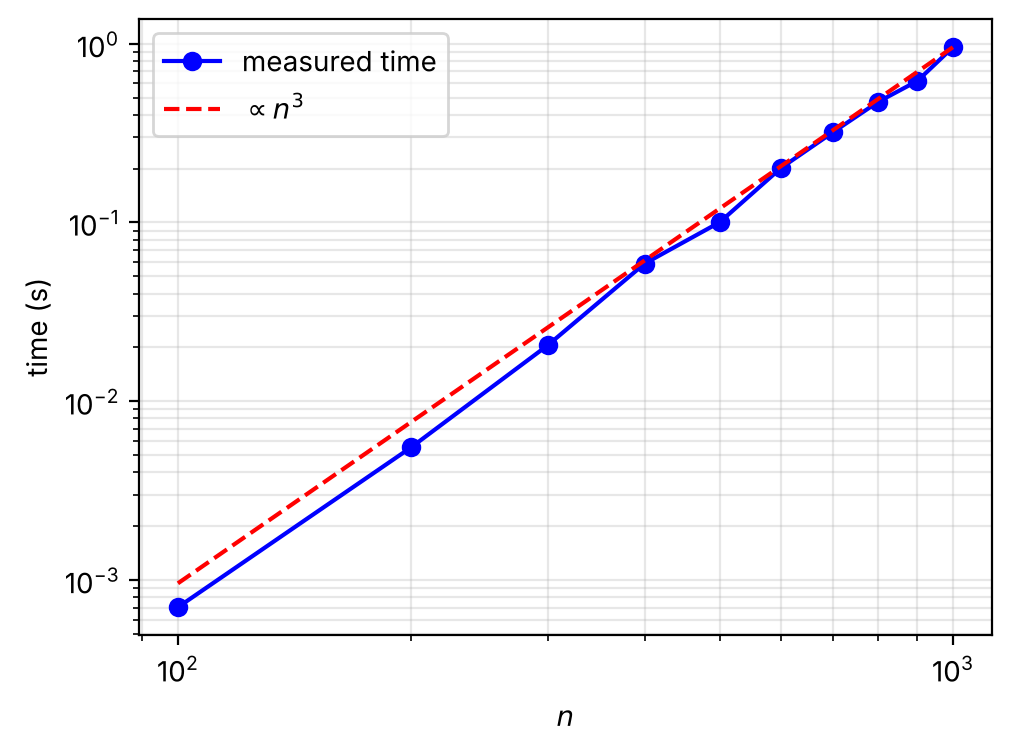
\includegraphics[width=0.8\linewidth]{figs/2.2.14b_time.png}
    \caption{Time of Gaussian elimination against $n$ (log-log), measured by the C program}
    \label{fig:gauss_time_q14}
\end{figure}
Both parts are verified in Python:
\codedesc{2.2.14a.py}{Applies the six row operations to $[A\,|\,I]$ with SymPy and compares the result with \texttt{A.inv()}, then row-reduces $[A\,|\,\vec{b}]$ for part (b).}
\begin{lstlisting}[frame=single, basicstyle=\rmfamily, escapeinside={(*@}{@*)}]
(*@\makebox[\dimexpr\linewidth-2\fboxsep-2\fboxrule\relax][c]{codes/2.2.14a.py}@*)
\end{lstlisting}
    \item
    \begin{enumerate}[label=(\alph*), leftmargin=1.5em, labelsep=0.5em]
        \item Using integration, find the area of the following region: $\{(x,y) : x^2+y^2\leq 16a^2 \text{ and } y^2\leq 6ax\}$

        \begin{center}
            \textbf{OR}
        \end{center}

        \item Using integration, find the area of triangle $ABC$ bounded by the lines $4x-y+5=0$, $x+y-5=0$ and $x-4y+5=0$.
    \end{enumerate} \vspace{2pt}

\par\hfill (12, 2018)\par
\textbf{(a) Solution:} Assume $a = 1$; for a general $a$ every length scales by $a$ and the area by $a^2$. Substituting $y^2 = 6x$ into $x^2 + y^2 = 16$, the curves meet where
\begin{align}
f(x) = x^2 + 6x - 16 = 0, \quad f'(x) = 2x + 6
\end{align}
Newton--Raphson \eqref{eq:12-newton} from $x_0 = 5$ gives
\begin{align*}
x_1 = 2.5625, \quad x_2 = 2.028441, \quad x_3 = 2.000080, \quad x_4 = 2.000000
\end{align*}
so $x = 2$ and $y = \pm\sqrt{12} = \pm 2\sqrt{3}$. The other root, $x = -8$, gives $y^2 < 0$ and is rejected. For each $y$ between the meeting points, the region runs from the parabola $x = \frac{y^2}{6}$ on the left to the circle $x = \sqrt{16 - y^2}$ on the right. The region is symmetric about the $x$-axis, so from \eqref{eq:EE26BTECH11225-area-curves-y},
\begin{align}
\text{Area} = 2\int_0^{2\sqrt{3}}\brak{\sqrt{16 - y^2} - \frac{y^2}{6}}dy
\end{align}
The two integrals are
\begin{align*}
\int_0^{2\sqrt{3}}\sqrt{16 - y^2}\,dy &= \sbrak{\frac{y}{2}\sqrt{16 - y^2} + 8\sin^{-1}\frac{y}{4}}_0^{2\sqrt{3}} \\
&= \sqrt{3}\cdot 2 + 8\cdot\frac{\pi}{3} = 2\sqrt{3} + \frac{8\pi}{3} \\
\int_0^{2\sqrt{3}}\frac{y^2}{6}\,dy &= \sbrak{\frac{y^3}{18}}_0^{2\sqrt{3}} = \frac{24\sqrt{3}}{18} = \frac{4\sqrt{3}}{3}
\end{align*}
so
\begin{align*}
\text{Area} = 2\brak{2\sqrt{3} + \frac{8\pi}{3} - \frac{4\sqrt{3}}{3}} = \frac{16\pi}{3} + \frac{4\sqrt{3}}{3} = \frac{4}{3}\brak{4\pi + \sqrt{3}} = 19.0646
\end{align*}
The trapezoidal rule \eqref{eq:EE26BTECH11225-trapezoid} with $N = 10^5$ intervals gives the same $19.0646$. For a general $a$,
\begin{align}
\boxed{\text{Area} = \frac{4a^2}{3}\brak{4\pi + \sqrt{3}} \text{ sq. units}}
\end{align}
\textbf{(b) Solution:} The vertices are found by solving the lines in pairs:
\begin{align*}
4x - y = -5,\ x + y = 5 &\implies 5x = 0 \implies B = (0, 5) \\
x + y = 5,\ x - 4y = -5 &\implies 5y = 10 \implies C = (3, 2) \\
4x - y = -5,\ x - 4y = -5 &\xrightarrow{R_2 \to R_2 - \frac{1}{4}R_1} -\tfrac{15}{4}y = -\tfrac{15}{4} \implies A = (-1, 1)
\end{align*}
The sides are $AB: y = 4x + 5$, $BC: y = 5 - x$ and $AC: y = \frac{x+5}{4}$. The triangle lies above $AC$, below $AB$ for $-1 \leq x \leq 0$ and below $BC$ for $0 \leq x \leq 3$. So
\begin{align}
\text{Area} = \int_{-1}^{0}\brak{4x + 5 - \frac{x+5}{4}}dx + \int_{0}^{3}\brak{5 - x - \frac{x+5}{4}}dx
\end{align}
Each integrand is linear, so the trapezoidal rule \eqref{eq:EE26BTECH11225-trapezoid} with one interval is exact. The integrand (the height of the triangle) is $0$ at $x = -1$ and $x = 3$, and at $x = 0$ it is $5 - \frac{5}{4} = \frac{15}{4}$. Hence
\begin{align}
\text{Area} = \frac{1}{2}\brak{0 + \frac{15}{4}}\cdot 1 + \frac{1}{2}\brak{\frac{15}{4} + 0}\cdot 3 = \frac{15}{8} + \frac{45}{8} = \boxed{\frac{15}{2} \text{ sq. units}}
\end{align}
The two regions are plotted in \figref{fig:area_q15}.
\codedesc{2.2.15.c}{Finds $x = 2$ by Newton--Raphson, then evaluates both areas with the trapezoidal rule.}
\begin{lstlisting}[frame=single, basicstyle=\rmfamily, escapeinside={(*@}{@*)}]
(*@\makebox[\dimexpr\linewidth-2\fboxsep-2\fboxrule\relax][c]{codes/2.2.15.c}@*)
\end{lstlisting}
\codedesc{2.2.15.py}{Repeats both integrals with NumPy and plots the region and the triangle.}
\begin{lstlisting}[frame=single, basicstyle=\rmfamily, escapeinside={(*@}{@*)}]
(*@\makebox[\dimexpr\linewidth-2\fboxsep-2\fboxrule\relax][c]{codes/2.2.15.py}@*)
\end{lstlisting}
\begin{figure}[H]
    \centering
    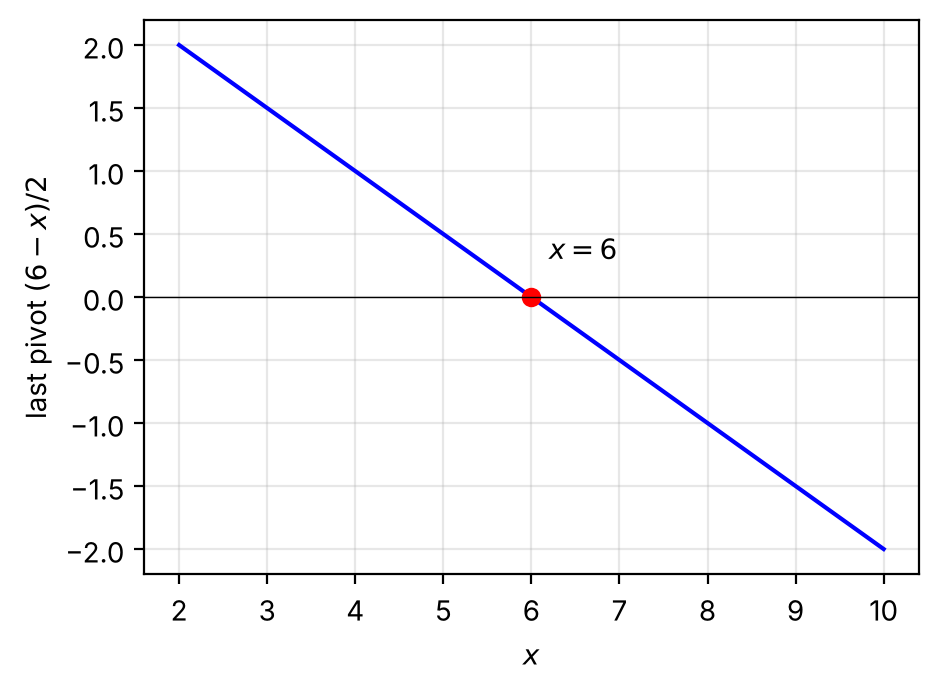
\includegraphics[width=\linewidth]{figs/2.2.15.png}
    \caption{(a) The region $x^2+y^2 \le 16$, $y^2 \le 6x$; (b) the triangle $ABC$}
    \label{fig:area_q15}
\end{figure}
    \item A company manufactures two types of novelty souvenirs made of plywood. Souvenirs of type A require 5 minutes each for cutting and 10 minutes each for assembling. Souvenirs of type B require 8 minutes each for cutting and 8 minutes each for assembling. There are 3 hours 20 minutes available for cutting and 4 hours for assembling. The profit for type A souvenirs is \rupee 100 each and for type B souvenirs, profit is \rupee 120 each. How many souvenirs of each type should the company manufacture in order to maximise the profit? Formulate the problem as a LPP and then solve it graphically.
\par\hfill (12, 2018)\par
\solution
Let $x$ and $y$ be the numbers of souvenirs of type A and B. Cutting takes $3$ h $20$ min $= 200$ min and assembling $4$ h $= 240$ min, so the cutting constraint is $5x + 8y \leq 200$ and the assembling constraint is $10x + 8y \leq 240$. In the form \eqref{eq:EE26BTECH11225-lpp},
\begin{align}
\max Z = \myvec{100 & 120}\myvec{x \\ y} \quad \text{s.t.} \quad \myvec{5 & 8 \\ 10 & 8}\myvec{x \\ y} \leq \myvec{200 \\ 240}, \quad x, y \geq 0
\end{align}
\textbf{Solving with CVXPY.} Let
\begin{align*}
\vec{x} = \myvec{x \\ y}, \quad \vec{c} = \myvec{100 \\ 120}, \quad \vec{A} = \myvec{5 & 8 \\ 10 & 8}, \quad \vec{b} = \myvec{200 \\ 240}
\end{align*}
The LPP is passed to CVXPY exactly as it is written above: one variable, one objective and a list of constraints.
\begin{lstlisting}[frame=single, language=Python, basicstyle=\ttfamily\footnotesize, columns=fullflexible]
import numpy as np
import cvxpy as cp
c = np.array([100, 120])
A = np.array([[5, 8], [10, 8]]); b = np.array([200, 240])
x = cp.Variable(2)                            # x = (x, y)
cons = [A @ x <= b, x >= 0]                   # cutting, assembling, x, y >= 0
prob = cp.Problem(cp.Maximize(c @ x), cons)   # maximise c^T x
prob.solve()
print(x.value, prob.value, cons[0].dual_value)
\end{lstlisting}
CVXPY returns
\begin{align}
\vec{x}^* = \myvec{8 \\ 20}, \quad Z_{\max} = \vec{c}^{\top}\vec{x}^* = 100(8) + 120(20) = \boxed{\text{\rupee}\,3200}
\end{align}
that is, $8$ souvenirs of type A and $20$ of type B. \\[4pt]
\textbf{Why this is the maximum.} CVXPY also returns the dual values $\bm{\lambda}$ of the two time constraints, which are the extra profit for one more minute of cutting and of assembling time:
\begin{align}
\bm{\lambda} = \myvec{10 \\ 5}
\end{align}
They satisfy $\bm{\lambda} \geq \vec{0}$ and $\vec{A}^{\top}\bm{\lambda} = \vec{c}$:
\begin{align*}
\myvec{5 & 10 \\ 8 & 8}\myvec{10 \\ 5} = \myvec{50 + 50 \\ 80 + 40} = \myvec{100 \\ 120}
\end{align*}
So for every feasible $\vec{x}$, from \eqref{eq:EE26BTECH11225-lpp-dual},
\begin{align*}
Z = \vec{c}^{\top}\vec{x} = \bm{\lambda}^{\top}\vec{A}\vec{x} \leq \bm{\lambda}^{\top}\vec{b} = 10(200) + 5(240) = 3200
\end{align*}
No production plan can earn more than \rupee\,3200, and $\vec{x}^*$ earns exactly that, so it is optimal. Both dual values are positive, so both constraints are tight at the optimum: $5(8) + 8(20) = 200$ and $10(8) + 8(20) = 240$, that is, all the cutting and assembling time is used. \\[4pt]
\textbf{Graphical check.} The feasible region in \figref{fig:lpp_q16} has the corners where the constraint lines meet the axes and each other:
\begin{align*}
10x + 8y = 240,\ y = 0 &\implies (24, 0) \\
5x + 8y = 200,\ x = 0 &\implies (0, 25) \\
(10x + 8y) - (5x + 8y) = 240 - 200 &\implies x = 8,\ y = \frac{200 - 40}{8} = 20
\end{align*}
(The other intercepts, $(40, 0)$ and $(0, 30)$, violate one of the constraints.) Evaluating $Z = 100x + 120y$ at each corner:
\[
\begin{array}{c|c}
\text{Corner} & Z \\\hline
(0, 0) & 0 \\
(24, 0) & 2400 \\
(8, 20) & 800 + 2400 = 3200 \\
(0, 25) & 3000
\end{array}
\]
The largest value is at $(8, 20)$, which agrees with CVXPY. The dashed line $Z = 3200$ in \figref{fig:lpp_q16} touches the region only at this corner.
\codedesc{2.2.16.py}{Sets up the LPP in CVXPY and solves it, prints $\vec{x}^*$, $Z_{\max}$ and the dual values $\bm{\lambda}$, checks $Z_{\max} = \vec{b}^{\top}\bm{\lambda}$, then evaluates $Z$ at the corner points and plots the feasible region.}
\begin{lstlisting}[frame=single, basicstyle=\rmfamily, escapeinside={(*@}{@*)}]
(*@\makebox[\dimexpr\linewidth-2\fboxsep-2\fboxrule\relax][c]{codes/2.2.16.py}@*)
\end{lstlisting}
\begin{figure}[H]
    \centering
    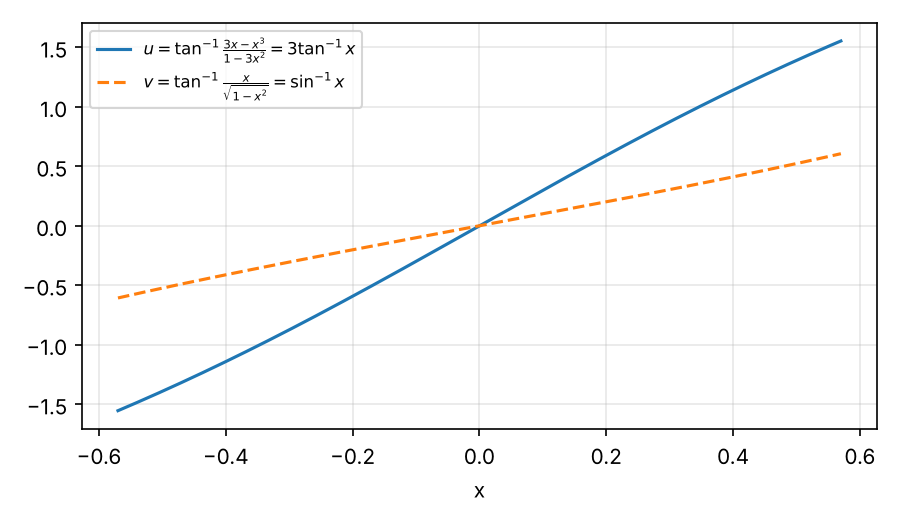
\includegraphics[width=0.75\linewidth]{figs/2.2.16.png}
    \caption{Feasible region and the optimum $(8,20)$}
    \label{fig:lpp_q16}
\end{figure}
    \item
    \begin{enumerate}[label=(\alph*), leftmargin=1.5em, labelsep=0.5em]
        \item Find the vector equation of the line passing through $(2,1,-1)$ and parallel to the line $\vec{r} = \myvec{1 \\ 1 \\ 0} + \lambda\myvec{2 \\ -1 \\ 1}$. Also, find the distance between these two lines.

        \begin{center}
            \textbf{OR}
        \end{center}

        \item Find the coordinates of the foot $Q$ of the perpendicular drawn from the point $P(1,3,4)$ to the plane $2x-y+z+3=0$. Find the distance $PQ$ and the image of $P$ treating the plane as a mirror.
    \end{enumerate} \vspace{2pt}

\par\hfill (12, 2018)\par
\textbf{(a) Solution:} A parallel line has the same direction $\vec{b} = \myvec{2 \\ -1 \\ 1}$, so the required line is
\begin{align}
\vec{x} = \myvec{2 \\ 1 \\ -1} + \mu\myvec{2 \\ -1 \\ 1}
\end{align}
Let $\vec{a}_1 = \myvec{1 \\ 1 \\ 0}$, $\vec{a}_2 = \myvec{2 \\ 1 \\ -1}$ and $\vec{w} = \vec{a}_2 - \vec{a}_1 = \myvec{1 \\ 0 \\ -1}$. From \eqref{eq:EE26BTECH11225-distance-lines}, the distance is the length of the part of $\vec{w}$ perpendicular to $\vec{b}$. With
\begin{align*}
\vec{b}^{\top}\vec{w} = 2(1) + (-1)(0) + 1(-1) = 1, \quad \vec{b}^{\top}\vec{b} = 4 + 1 + 1 = 6
\end{align*}
this part is
\begin{align*}
\vec{w} - \frac{\vec{b}^{\top}\vec{w}}{\vec{b}^{\top}\vec{b}}\vec{b} = \myvec{1 \\ 0 \\ -1} - \frac{1}{6}\myvec{2 \\ -1 \\ 1} = \myvec{\frac{2}{3} \\ \frac{1}{6} \\ -\frac{7}{6}}
\end{align*}
and its length is
\begin{align}
d = \sqrt{\frac{4}{9} + \frac{1}{36} + \frac{49}{36}} = \sqrt{\frac{16 + 1 + 49}{36}} = \sqrt{\frac{66}{36}} = \boxed{\sqrt{\frac{11}{6}}}
\end{align}
\textbf{(b) Solution:} The plane is $\vec{n}^{\top}\vec{x} = -3$ with $\vec{n} = \myvec{2 \\ -1 \\ 1}$, and $\vec{P} = \myvec{1 \\ 3 \\ 4}$. The quantities in \eqref{eq:EE26BTECH11225-foot} are
\begin{align*}
\vec{n}^{\top}\vec{P} = 2 - 3 + 4 = 3, \quad \norm{\vec{n}}^2 = 4 + 1 + 1 = 6, \quad t = \frac{-3 - 3}{6} = -1
\end{align*}
The foot of the perpendicular is
\begin{align}
\vec{Q} = \vec{P} + t\vec{n} = \myvec{1 \\ 3 \\ 4} - \myvec{2 \\ -1 \\ 1} = \boxed{\myvec{-1 \\ 4 \\ 3}}
\end{align}
the distance is
\begin{align}
PQ = \norm{\vec{Q} - \vec{P}} = |t|\norm{\vec{n}} = \boxed{\sqrt{6}}
\end{align}
and the image is twice as far along the normal:
\begin{align}
\vec{P}' = \vec{P} + 2t\vec{n} = \myvec{1 \\ 3 \\ 4} - 2\myvec{2 \\ -1 \\ 1} = \boxed{\myvec{-3 \\ 5 \\ 2}}
\end{align}
Check: $\vec{Q}$ is on the plane, since $2(-1) - 4 + 3 + 3 = 0$, and it is the midpoint of $PP'$. Both parts are plotted in \figref{fig:lines_q17}.
\codedesc{2.2.17.py}{Computes the distance between the lines by projection, and the foot $Q$ and the image $P'$, checks them, and plots both parts in 3D.}
\begin{lstlisting}[frame=single, basicstyle=\rmfamily, escapeinside={(*@}{@*)}]
(*@\makebox[\dimexpr\linewidth-2\fboxsep-2\fboxrule\relax][c]{codes/2.2.17.py}@*)
\end{lstlisting}
\begin{figure}[H]
    \centering
    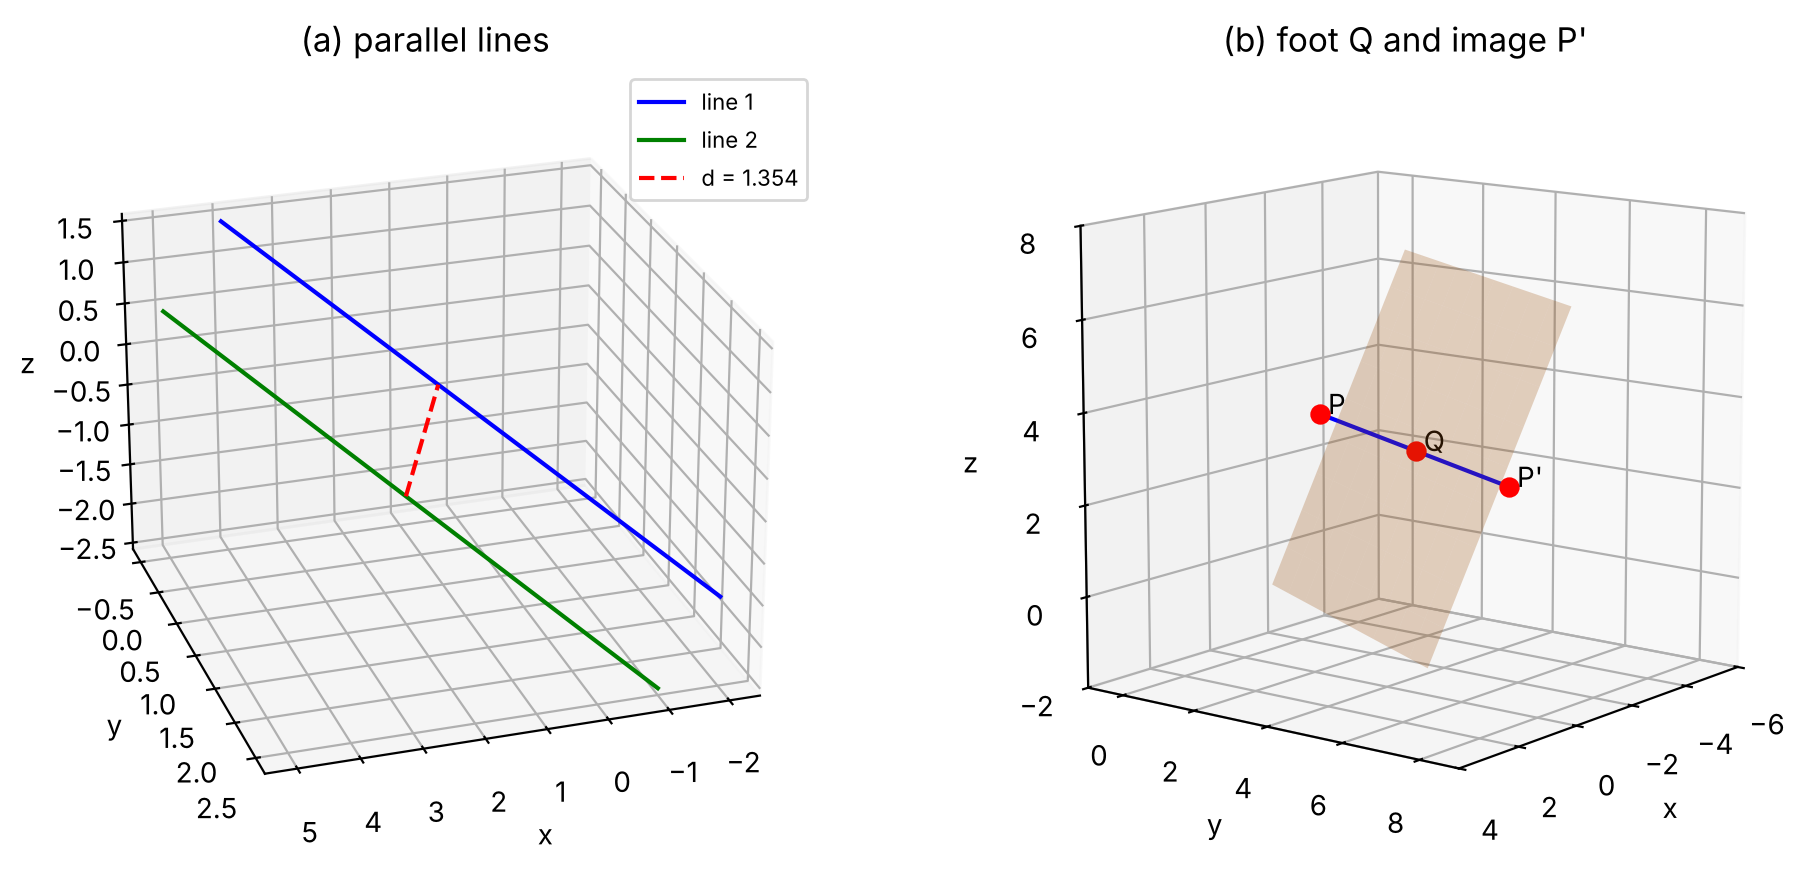
\includegraphics[width=\linewidth]{figs/2.2.17.png}
    \caption{(a) The parallel lines; (b) the foot $Q$ and the image $P^{\prime}$}
    \label{fig:lines_q17}
\end{figure}
    \item A card from a pack of 52 playing cards is lost. From the remaining cards of the pack, two cards are drawn at random (without replacement) and both are found to be spades. Find the probability of the lost card being a spade.
\par\hfill (12, 2018)\par
\solution
Let $L = 1$ if the lost card is a spade and $L = 0$ otherwise, and let $A$ be the event that both cards drawn from the remaining $51$ are spades. Since $13$ of the $52$ cards are spades, the prior pmf is
\begin{align*}
p_L(l) = \brak{\frac{1}{4}}^l\brak{\frac{3}{4}}^{1-l}
\end{align*}
If the lost card is a spade, $12$ spades remain among the $51$ cards; otherwise all $13$ remain. So the likelihood of drawing two spades is
\begin{align*}
p_{A|L}(l) = \frac{\binom{13-l}{2}}{\binom{51}{2}}, \quad \binom{12}{2} = 66, \quad \binom{13}{2} = 78
\end{align*}
By Bayes' theorem (using \eqref{eq:12-pmf} to normalise), the posterior pmf is $p_{L|A}(l) \propto p_L(l)\,p_{A|L}(l)$. The common factor $\binom{51}{2}$ cancels, so
\begin{align}
p_{L|A}(1) = \frac{\frac{1}{4}\binom{12}{2}}{\frac{1}{4}\binom{12}{2} + \frac{3}{4}\binom{13}{2}} = \frac{66}{66 + 3 \times 78} = \frac{66}{300} = \boxed{\frac{11}{50}}
\end{align}
\figref{fig:pmf_q18} compares the simulated posterior with the theoretical one.
\codedesc{2.2.18.py}{Computes the posterior with Bayes' theorem, simulates by shuffling a pack, and compares the two in a stem plot.}
\begin{lstlisting}[frame=single, basicstyle=\rmfamily, escapeinside={(*@}{@*)}]
(*@\makebox[\dimexpr\linewidth-2\fboxsep-2\fboxrule\relax][c]{codes/2.2.18.py}@*)
\end{lstlisting}
\begin{figure}[H]
    \centering
    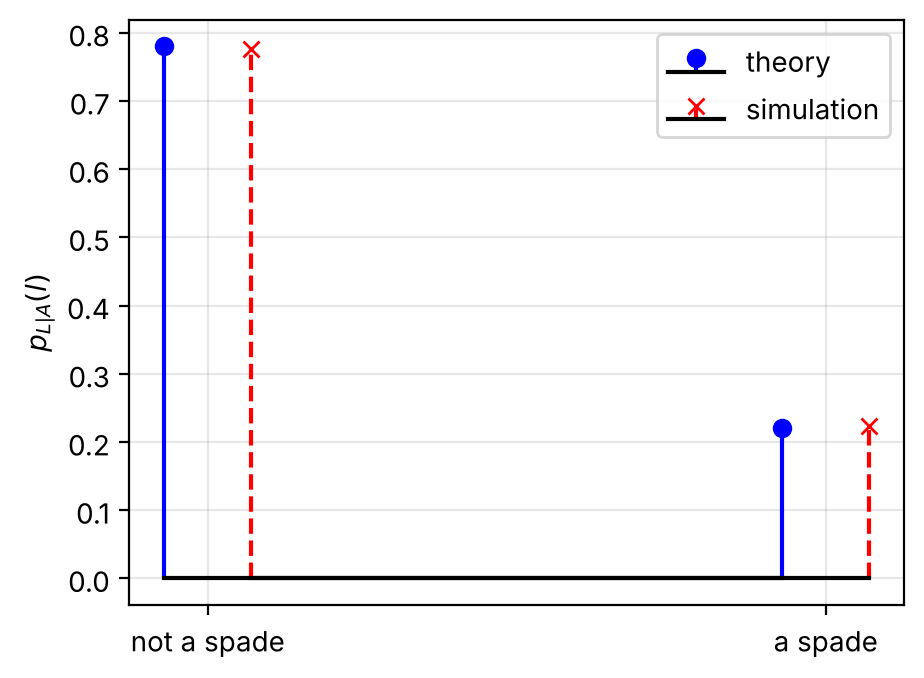
\includegraphics[width=0.7\linewidth]{figs/2.2.18.png}
    \caption{Theoretical and simulated $p_{L|A}(l)$}
    \label{fig:pmf_q18}
\end{figure}
\end{enumerate}
